% !Mode::"TeX:UTF-8"
%%%%%%%%%%%%%%%%%%%%%%%%%%%%%%%%%%%%%%%%%%%%%%%%%%%%%%%%%%%%%%%%%%%%%%%%%%%%%
%%%     这是一份 beamer 文档. 本源文件仅供学习 beamer 参考之用.           %%%
%%%     使用请注明出处. 本文作者拥有版权 (c)2014. 保留所有权利.           %%%
%%%                                                                       %%%
%%%     使用XeLaTeX直接编译即可,注意打开时的编码方式为UTF-8 ^_^          %%%
%%%     作者: 李泽魁 (http://ir.hit.edu.cn/~zkli/)  2014-01-06            %%%
%%%                                                                       %%%
%%%          感谢Slides最后参考文献中的诸多大牛们的无私奉献!             %%%
%%%                       共同学习,共同进步!                            %%%
%%%%%%%%%%%%%%%%%%%%%%%%%%%%%%%%%%%%%%%%%%%%%%%%%%%%%%%%%%%%%%%%%%%%%%%%%%%%%

\documentclass[notheorems]{beamer}
\usepackage[UTF8,noindent]{ctex}
\usepackage[english]{babel}   %如果去掉,中英混合会出错
\usepackage{amsmath,amssymb,amsfonts}
\usepackage{tikz}
\usetheme{Madrid}
\usepackage{graphicx}                          % 比graphics先进
\usepackage{subfigure}                         % 子图并排
\usepackage{picins}                            % 图片嵌入段落宏包 比如照片
\usepackage{verbatim}                          % 照写区
\usepackage{listings}                          % 代码
\usepackage{xcolor}                            % 使用颜色宏包
\usepackage{algorithm}                         % format of the algorithm
\usepackage{algorithmic}
\usepackage{xltxtra}                           %logos
\usepackage{mflogo,texnames}


\graphicspath{{images/}}                       %图片路径

%==============自定义: 逐个 item 高亮(\hilite), 或"高黑"(\hidark)==================%
\def\hilite<#1>{%
\temporal<#1>{\color{blue!35}}{\color{magenta}}%
{\color{blue!75}}}
\def\hidark<#1>{%
\temporal<#1>{\color{black!35}}{\color{magenta}}%
{\color{black}}}

%====================== metapost =================================================%
\usepackage{xmpmulti}  %% metapost 动画.
\DeclareGraphicsRule{*}{mps}{*}{}


\begin{document}
%%-------------------------------------------------
\title{\LaTeX~入门}
\author[zkli]{\href{http://ir.hit.edu.cn/~zkli/}{zkli}\\[0.5em]{\color{blue!70}\texttt{zkli@ir.hit.edu.cn}}\\}
\institute[哈尔滨工业大学~SCIR研究中心]{\kaishu\textcolor{olive}{\href{http://www.hit.edu.cn/}{哈尔滨工业大学}~~\href{http://ir.hit.edu.cn/}{SCIR研究中心}}}
\date{}
\titlegraphic{
\includegraphics[height=2cm]{hit_logo}\qquad 
\includegraphics[height=1.8cm]{scir_logo}}
\frame{\titlepage}
%%-------------------------------------------------

\begin{frame}\frametitle{目录}\small
\tableofcontents
\end{frame}
%************************************************
\section{\LaTeX{}是什么}
\begin{frame}
    \frametitle{\TeX{}}
    \begin{itemize}
        \hidark<1> \item 由Donald E. Knuth (高德纳,唐纳德·克努特) 1977年开始设计
        \hidark<2> \item 由三个希腊字母组成,发音为“Tech”(泰克)
        \hidark<3> \item 最初用于出版工业的数字印刷设备
        \hidark<4> \item 从第3版之后的版本号越来越接近圆周率$\pi$ ,目前的版本是3.1415926
        \hidark<5> \item 非常稳定,高德纳悬赏奖励任何能够在\TeX{}中发现程序漏洞(bug)的人
    \end{itemize}
\end{frame}

\begin{frame}\frametitle{高德纳的传奇}
    \begin{columns}

    	\begin{column}{0.3\textwidth}
        	\begin{figure}[h]
                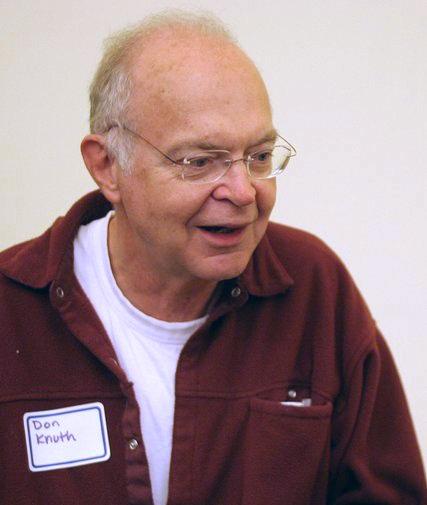
\includegraphics[width=0.9\textwidth]{donald.jpg}
                \caption{高公萌照}
            \end{figure}
    	\end{column}

    	\begin{column}{0.7\textwidth}
        	\begin{itemize}
                \hidark<1> \item 《The Art of Computer Programming》作者
                \hidark<2> \item  美国国家科学院院士
                \hidark<3> \item  美国工程院院士
                \hidark<4> \item  美国艺术与科学院院士
                \hidark<5> \item  斯坦福大学计算机系教授(30岁)
                \hidark<6> \item  最年轻的图灵奖获得者(36岁)
            \end{itemize}
    	\end{column}

    \end{columns}


    \begin{center}
        \footnotesize{\url{http://www-cs-faculty.stanford.edu/~knuth/}}
    \end{center}

\end{frame}

\begin{frame}\frametitle{\LaTeX{}}
    \begin{itemize}
        \hidark<1> \item 发音为“Lay-Tech”(雷态克)
        \hidark<2> \item 由最早由计算机学家Lamport在20世纪80年代初开发
        \hidark<3> \item \LaTeX{} 是在Plain \TeX{}的基础上开发出的一种更为简单的语言
        \hidark<4> \item 提供了预先定义好的专业页面设置
        \hidark<5> \item 短时间内生成具有书籍质量的印刷品
        \hidark<6> \item 还可以用来生成矢量图形
    \end{itemize}
\end{frame}

\begin{frame}\frametitle{\LaTeX{}优点}
    \begin{itemize}
        \item<1-> \textcolor{red}{模板漂亮}。让你的文档足够漂亮以应对各种场合-
        \item<2-> \textcolor{red}{编写方便}。可以容易地编辑公式、生成脚注、索引、目录、参考文献等复杂的文档结构
        \item<3-> \textcolor{red}{省时省力}。可以免去很多费力不讨好的页面样式设计工作
        \item<4-> \textcolor{red}{资源丰富}。有大量的模版可以借鉴,很容易套用
        \item<5-> \textcolor{red}{统一标准}。\LaTeX{}是科研界标准,很多期刊提供模板,甚至提供在线编译功能
        \item<6-> \textcolor{red}{当前国情}。用\LaTeX{}写算法导论报告分数会高一些
        \item<7-> \textcolor{red}{业界良心}。体会码农的乐趣
    \end{itemize}
\end{frame}

\begin{frame}\frametitle{\LaTeX{}缺点}
    \begin{itemize}
        \hidark<1> \item 不是所见即所得,上手不如word简单,但是一劳永逸。
        %有人把时间花在了重复工作上,有人花了积累模板上。一两年以后,前者依旧,后者不再需要花时间。
        \hidark<2> \item 组织结构混乱的文章不太容易写,但我们追求的就是清晰的结构。
        \hidark<3> \item 自己重新设计整个排版很花时间,但我们没有设计排版的需求。
        \hidark<4> \item 很难做出很花哨的效果,但我们不会去做花哨的效果。
    \end{itemize}
\end{frame}

\begin{frame}\frametitle{\LaTeX{} vs Word}{——能抓到老鼠的猫就是好猫}
    \begin{figure}[h]
        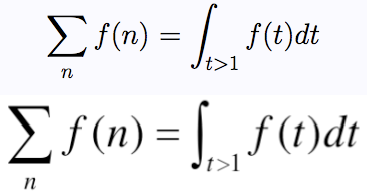
\includegraphics[width=0.4\textwidth]{latex_word.png}
    \end{figure}
    \begin{itemize}
        \hidark<2> \item \LaTeX{}各种字母体型优美,仪态万方
        \hidark<3> \item 文档大小较之Word小很多,并且是文本格式
    \end{itemize}
\end{frame}

\begin{frame}\frametitle{接下来要介绍的内容}
    \begin{itemize}
        \hidark<1> \item helloworld.tex
        \hidark<2> \item 基本语法介绍
        \hidark<3> \item 章节、段落
        \hidark<4> \item 数学公式
        \hidark<5> \item 插入代码、图片、表格和引用
        \hidark<6> \item 中文支持
        \hidark<7> \item Beamer(Slides NOT PPT)
        \hidark<8> \item 参考文献的加入
        \hidark<9> \item 几个省事的软件
    \end{itemize}
\end{frame}

%************************************************
\section{helloworld.tex}
\begin{frame}\frametitle{准备工作}
    \begin{itemize}
        \item TEX套装
            \begin{itemize}
        		\item Windows:MiKTeX, \textcolor{red}{CTeX}
        		\item Linux:teTEX
        		\item 跨平台:\textcolor{red}{TeX Live}, MacTeX, ConTeXt
        	\end{itemize}
        \item 编译器
            \begin{itemize}
        		\item Windows:TeXnicCenter, MeWa, WinShell, BakoMa TeX, Inlage, \textcolor{red}{WinEdt}, \ldots
        		\item Linux:Gedit LaTeX Plugin, Gummi, Winefish, \textcolor{red}{Kile}, \ldots
        		\item 跨平台:\textcolor{red}{LyX}, Texmaker, AUCTEX, TeXlipse, \textcolor{red}{TeXworks}, \ldots
        		\item 详细比较:\\http://en.wikipedia.org/wiki/Comparison\_of\_TeX\_editors
        		\item vim和emacs可以通过相应插件来支持\LaTeX
        	\end{itemize}
    \end{itemize}
\end{frame}

\begin{frame}\frametitle{编译过程}
    \begin{figure}[t]
        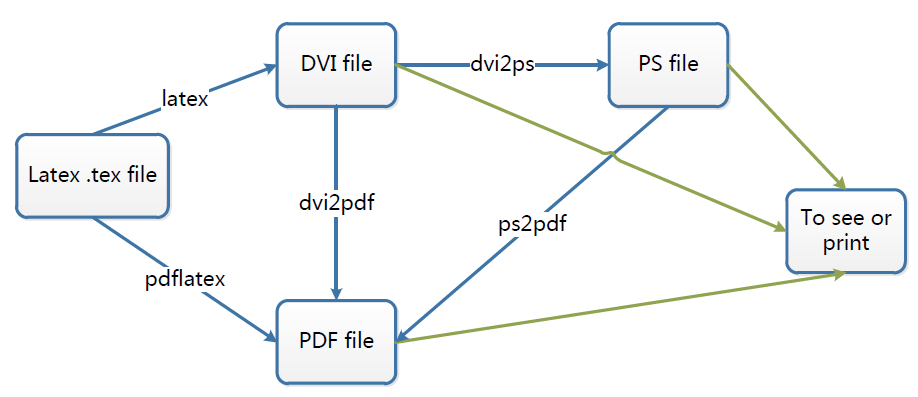
\includegraphics[width=0.8\textwidth]{compile_procedure.png}
    \end{figure}
    \begin{block}{}
        \center
      其中DVI、PostScript和PDF为三种输出格式。
    \end{block}
\end{frame}



\begin{frame}[fragile]
\frametitle{动手写一个hello \LaTeX{}}
    \begin{block}{HelloLatex.tex}
    \begin{verbatim}
% !Mode:: "TeX:UTF-8"
\documentclass{article}
\author{fool}
\title{My First \LaTeX{} article}

\begin{document}
\maketitle
    Wow! This is my FIRST \LaTeX{} Article!

    Hello World!
\end{document}
    \end{verbatim}
    \end{block}
\end{frame}

\begin{frame}[fragile]\frametitle{基本语法介绍}
    \begin{itemize}
        \hidark<1> \item 空格:连续的空格被认为只有一个,用\verb|~|表示空格
        \hidark<2> \item 有些特殊的符号是不能直接使用的:\\
                    \verb|$ & % # _ { }|
                    应该写成
                    \verb|\$ \& \% \# \_ \{ \}|
        \hidark<3> \item 断行:\verb|\\|
        \hidark<4> \item 分段:文字之后的一个空行是段落结束的标志
        \hidark<5> \item 注释:\verb|%|之后都文字都是注释,是无效的语句
        \hidark<6> \item LaTeX的命令:以\verb|\|开始: \\
                    \begin{verbatim}
    \section{第一段}
    \emph{强调}
                   \end{verbatim}
    \end{itemize}
\end{frame}

%************************************************
\section{章节、段落}
\begin{frame}[fragile]\frametitle{章节、段落}
    \begin{itemize}
      \item<1->in article:
        \begin{itemize}
              \item<2->  \textbackslash section\{section name\}
              \item<3->  \textbackslash subsection\{subsection name\}
              \item<4->  \textbackslash paragraph\{paragraph name\}
              \item<5->  \textbackslash subparagraph\{subparagraph name\}
        \end{itemize}
      \item<6->in book:
        \begin{itemize}
              \item<7->  \textbackslash chapter\{chapter name\}
              \item<8->  \textbackslash part\{part name\}
        \end{itemize}
      \item<9->in beamer:
        \begin{itemize}
              \item<10->  \textbackslash section\{section name\}
        \end{itemize}
    \end{itemize}
\end{frame}


%************************************************
\section{数学公式}
\begin{frame}[fragile]\frametitle{传说中的方便插入公式?}
article中的两种公式:
    \begin{itemize}
      \hidark<1> \item 行内公式(inline mode)
        \begin{itemize}
          \hidark<2> \item \textbackslash ( \ldots \textbackslash )
		  \hidark<3> \item \textbackslash begin\{math\} \ldots \textbackslash end\{math\}
		  \hidark<4> \item \$ \ldots \$
        \end{itemize}
      \hidark<5> \item 行间公式(display mode)
        \begin{itemize}
          \hidark<6> \item \textbackslash begin\{equation\} \ldots \textbackslash end\{equation\}
		  \hidark<7> \item \textbackslash [ \ldots \textbackslash ]
		  \hidark<8> \item \textbackslash begin\{displaymath\} \ldots \textbackslash end\{displaymath\}
		  \hidark<9> \item \$\$ \ldots \$\$
        \end{itemize}
      \hidark<10> \item 多行公式
    \end{itemize}
\end{frame}

\begin{frame}[fragile]\frametitle{用例子说明两种公式的区别}
    \begin{block}{Input}
    \begin{verbatim}
I know that you know $1+1=2$, but I know $2-1=1$, which you
don't know. Now look at it $$2-1=1$$ I DO know more than you
    \end{verbatim}
    \end{block}
    \begin{block}{Output}
        I know that you know $1+1=2$, but I know $2-1=1$, which you don't know. Now look at it $$2-1=1$$ I DO know more than you.
    \end{block}
\end{frame}

\begin{frame}[fragile]\frametitle{分式、上下标和开方}
    \begin{block}{Input}
    \begin{verbatim}
$$\frac{2011}{2012}, x_1,x_2,\ldots,x_n, a^2+b^2=c^2,
x_1^2+x_2^2+\ldots+x_n^2=r^{100}, \sqrt{x+1},
\sqrt[3]{x^2+1}$$
    \end{verbatim}
    \end{block}
    \begin{block}{Output}
        $$\frac{2011}{2012}, x_1,x_2,\ldots,x_n, a^2+b^2=c^2, x_1^2+x_2^2+\ldots+x_n^2=r^{100}, \sqrt{x+1}, \sqrt[3]{x^2+1}$$
    \end{block}
\end{frame}

\begin{frame}[fragile]\frametitle{三角函数}
    \begin{block}{Input}
    \begin{verbatim}
$$\sin x, \cos x, \tan x, \arctan x, \sinh x, \cosh x,
\max x, \min x, \ln x, \log x, \log_2 x.$$
    \end{verbatim}
    \end{block}
    \begin{block}{Output}
        $$\sin x, \cos x, \tan x, \arctan x, \sinh x, \cosh x, \max x, \min x
        , \ln x, \log x, \log_2 x.$$
    \end{block}
\end{frame}

\begin{frame}[fragile]\frametitle{求和、极限和积分}
    \begin{block}{Input}
    \begin{verbatim}
$$\lim_{n \to \infty} a_n = 1, \sum_{n=1}^{\infty} n = 5050,
\int_{a}^{b}f(x) \mathrm{d}x = I$$
    \end{verbatim}
    \end{block}
    \begin{block}{Output}
        $$\lim_{n \to \infty} a_n = 1, \sum_{n=1}^{\infty} n = 5050,
        \int_{a}^{b}f(x) \mathrm{d}x = I$$
    \end{block}
\end{frame}

\begin{frame}[fragile]\frametitle{关系符号、希腊字母和部分数学标记}
    \begin{block}{Input}
    \begin{verbatim}
$$a \times b, c \div d, a<b , b=c, c \neq d, d > e,
e \geq f, f \leq g $$
$$\alpha\beta\gamma\delta\epsilon\varepsilon\xi\pi
\rho\sigma\eta\theta\phi\varphi\omega$$
$$|A|, \|A\|, \vec{a}, \overrightarrow{AB}, \tilde{x},
\widetilde{xyz}, \mathrm{sin}$$
    \end{verbatim}
    \end{block}
    \begin{block}{Output}
        $$a \times b, c \div d, a<b , b=c, c \neq d, d > e, e \geq f, f \leq g $$
        $$\alpha\beta\gamma\delta\epsilon\varepsilon\xi\pi\rho\sigma\eta
        \theta\phi\varphi\omega ,|A|, \|A\|, \vec{a}, \overrightarrow{AB}, \tilde{x},
        \widetilde{xyz}, \mathrm{sin}$$
    \end{block}
\end{frame}

\begin{frame}[fragile]\frametitle{矩阵}
  \begin{columns}
    \begin{column}{0.05\textwidth}
    \end{column}
    \begin{column}{0.45\textwidth}
    \begin{block}{Input}
    \begin{verbatim}
\begin{equation}
\left(
\begin{array}{ccc}
a_{11} & a_{12} & a_{13} \\
a_{21} & a_{22} & a_{23} \\
a_{31} & a_{32} & a_{33}
\end{array}
\right)
\end{equation}
    \end{verbatim}
    \end{block}
    \end{column}
    \begin{column}{0.025\textwidth}
    \end{column}
    \begin{column}{0.45\textwidth}
    \begin{block}{Output}
        \begin{equation}
        \left(
        \begin{array}{ccc}
        a_{11} & a_{12} & a_{13} \\
        a_{21} & a_{22} & a_{23} \\
        a_{31} & a_{32} & a_{33}
        \end{array}
        \right)
        \end{equation}
    \end{block}
    \end{column}
    \begin{column}{0.025\textwidth}
    \end{column}
  \end{columns}
\end{frame}

\begin{frame}[fragile]\frametitle{矩阵v2.0}
  \begin{columns}
    \begin{column}{0.05\textwidth}
    \end{column}
    \begin{column}{0.45\textwidth}
    \begin{block}{Input}
    \begin{verbatim}
\begin{equation}
\left\{
\begin{array}{c||c|c}
a_{11} & a_{12} & \\
\hline
a_{21} & & a_{23} \\
& a_{32} & a_{33}
\end{array}
\right)
\end{equation}
    \end{verbatim}
    \end{block}
    \end{column}
    \begin{column}{0.025\textwidth}
    \end{column}
    \begin{column}{0.45\textwidth}
    \begin{block}{Output}
        \begin{equation}
        \left\{
        \begin{array}{c||c|c}
        a_{11} & a_{12} & \\
        \hline
        a_{21} & & a_{23} \\
        & a_{32} & a_{33}
        \end{array}
        \right)
        \end{equation}
    \end{block}
    \end{column}
    \begin{column}{0.025\textwidth}
    \end{column}
  \end{columns}
\end{frame}

\begin{frame}[fragile]\frametitle{分段函数}
  \begin{columns}
    \begin{column}{0.05\textwidth}
    \end{column}
    \begin{column}{0.45\textwidth}
    \begin{block}{Input}
    \begin{verbatim}
\begin{equation}
\chi_A(x)=
\left\{
\begin{array}{ll}
1, & x \in A \\
0, & x \not\in A
\end{array}
\right.
\end{equation}
    \end{verbatim}
    \end{block}
    \end{column}
    \begin{column}{0.025\textwidth}
    \end{column}
    \begin{column}{0.45\textwidth}
    \begin{block}{Output}
        \begin{equation}
        \chi_A(x)=
        \left\{
        \begin{array}{ll}
        1, & x \in A \\
        0, & x \not\in A
        \end{array}
        \right.
        \end{equation}
    \end{block}
    \end{column}
    \begin{column}{0.025\textwidth}
    \end{column}
  \end{columns}
\end{frame}

%************************************************
\section{算法、代码、表格、图片和引用}
\begin{frame}[fragile]\frametitle{插入算法v1.0}
  \begin{columns}
    \begin{column}{0.05\textwidth}
    \end{column}
    \begin{column}{0.45\textwidth}
    \begin{block}{Input}
    \begin{verbatim}
\begin{algorithm}[H]
\caption{An Algorithm}
\begin{algorithmic}[1]
\FOR{each $i in [1,9]$}
\STATE initialize $T_{i}$;\
\STATE $T_{i};$\
\ENDFOR
\end{algorithmic}
\end{algorithm}
    \end{verbatim}
    \end{block}
    \end{column}
    \begin{column}{0.025\textwidth}
    \end{column}
    \begin{column}{0.45\textwidth}
    \begin{block}{Output}
\begin{algorithm}[H]
\caption{An Algorithm}
\begin{algorithmic}[1]
\FOR{each $i in [1,9]$}
\STATE initialize $T_{i}$;\
\STATE $T_{i};$\
\ENDFOR
\end{algorithmic}
\end{algorithm}
    \end{block}
    \end{column}
    \begin{column}{0.025\textwidth}
    \end{column}
  \end{columns}
\end{frame}

\begin{frame}[fragile]\frametitle{插入算法v2.0}
  \begin{columns}
    \begin{column}{0.05\textwidth}
    \end{column}
    \begin{column}{0.45\textwidth}
    \begin{block}{Input}
    \begin{verbatim}
\begin{algorithm}[H]
\caption{Description}
\begin{algorithmic}[1]
\REQUIRE ~~\\
The samples, $P_n$;\\
\ENSURE ~~\\
Classifiers, $E_n$;\\
\STATE Samples $T_n$;
\STATE Classifiers $E$
\end{algorithmic}
\end{algorithm}
    \end{verbatim}
    \end{block}
    \end{column}
    \begin{column}{0.025\textwidth}
    \end{column}
    \begin{column}{0.45\textwidth}
    \begin{block}{Output}
\begin{algorithm}[H]
\caption{Description}
\begin{algorithmic}[1]
\REQUIRE ~~\\
The samples, $P_n$;\\
\ENSURE ~~\\
Classifiers, $E_n$;\\
\STATE Samples $T_n$;
\STATE Classifiers $E$
\end{algorithmic}
\end{algorithm}
    \end{block}
    \end{column}
    \begin{column}{0.025\textwidth}
    \end{column}
  \end{columns}
\end{frame}

\begin{frame}[fragile]\frametitle{插入代码v1.0}
  \begin{columns}
    \begin{column}{0.05\textwidth}
    \end{column}
    \begin{column}{0.45\textwidth}
    \begin{block}{Input}
    \begin{verbatim}
\usepackage{listings}
\begin{lstlisting}
[language=C]
int main(void)
{
printf("Hello world!\n");
return 0;
}
\end{lstlisting}
    \end{verbatim}
    \end{block}
    \end{column}
    \begin{column}{0.025\textwidth}
    \end{column}
    \begin{column}{0.45\textwidth}
\begin{lstlisting}[language=C]
int main(void)
{
printf("Hello world!\n");
return 0;
}
\end{lstlisting}
    \end{column}
    \begin{column}{0.025\textwidth}
    \end{column}
  \end{columns}
\end{frame}

\begin{frame}[fragile]\frametitle{插入代码v6.0}
  \begin{columns}
    \begin{column}{0.005\textwidth}
    \end{column}
    \begin{column}{0.425\textwidth}
    \begin{block}{Input}
    \begin{verbatim}
\lstset
{numbers=left,blarblar}
\begin{lstlisting}
[language=C]
int main(void)
{
printf("Hello world!\n");
return 0;
}
\end{lstlisting}
    \end{verbatim}
    \end{block}
    \end{column}
    \begin{column}{0.025\textwidth}
    \end{column}
    \begin{column}{0.52\textwidth}
\begin{lstlisting}[language=C, numbers=left,
numberstyle=\tiny, keywordstyle=\color{blue!70}, commentstyle=\color{red!50!green!50!blue!50},
frame=shadowbox, rulesepcolor=\color{red!20!green!20!blue!20}]
int main(void)
{
/* print a string*/
printf("Hello world!\n");
return 0;
}
\end{lstlisting}
    \end{column}
    \begin{column}{0.025\textwidth}
    \end{column}
  \end{columns}
\end{frame}

\begin{frame}[fragile]\frametitle{插入表格}
  \begin{columns}
    \begin{column}{0.05\textwidth}
    \end{column}
    \begin{column}{0.45\textwidth}
    \begin{block}{Input}
    \begin{verbatim}
\begin{tabular}{l|l}
Name & score \\
\hline
You & 100 \\
Me & 59
\end{tabular}
    \end{verbatim}
    \end{block}
    \end{column}
    \begin{column}{0.05\textwidth}
    \end{column}
    \begin{column}{0.40\textwidth}
    \begin{block}{Output}
        \begin{tabular}{l|l}
        Name & score \\
        \hline
        You & 100 \\
        Me & 59
        \end{tabular}
    \end{block}
    \end{column}
    \begin{column}{0.05\textwidth}
    \end{column}
  \end{columns}
\end{frame}

\begin{frame}[fragile]\frametitle{图片格式支持什么?}
    \begin{description}
		\item[ps]: PostScript. 由Adobe公司推出,是一种页面描述语言。独立于设备,能综合处理文字和图像,擅长于描述矢量图形。
		\item[eps]: Encapsulated PostScript. 封装的PostScript,是PostScript的一个子集,每个eps文件只有一个页面。eps格式的图片与\LaTeX 最兼容。
        \item[pdf]: Portable Document Format
		\item[非矢量图]:jpg, png, bmp, \ldots : 各种其他图片格式,也被\LaTeX 支持
	\end{description}
\end{frame}

\begin{frame}[fragile]\frametitle{插入jpg图片}
   \begin{block}{Input}
    \begin{verbatim}
\begin{figure}[h]
    \centering
    
\includegraphics[width=0.3\textwidth,angle=20]{jpg_figure}
\end{figure}
    \end{verbatim}
   \end{block}
   \begin{figure}[h]
    \centering
    
\includegraphics[width=0.3\textwidth,angle=20]{jpg_figure}
   \end{figure}
\end{frame}

%看源码的同学,这里我要说明下,本来想做个eps的例子,但是由于这个beamer是pdflatex编译的(最初2了)
%如果要编译eps,需要用latex 或 xelatex
\begin{frame}[fragile]\frametitle{矢量图vs非矢量图}
    \begin{center}
    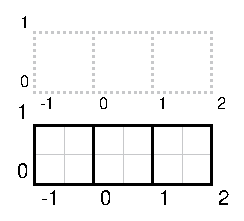
\includegraphics[height=0.3\textwidth]{eps_figure.eps}\qquad
    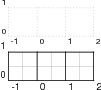
\includegraphics[height=0.3\textwidth]{png_figure.png}
    \end{center}
\end{frame}


\begin{frame}[fragile]\frametitle{插入eps图片}
   \begin{block}{Input}
    \begin{verbatim}
    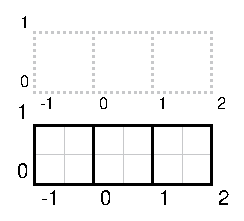
\includegraphics[width=0.5\textwidth]{eps_figure.eps}
    \end{verbatim}
   \end{block}
   \begin{figure}[h]
    \centering
    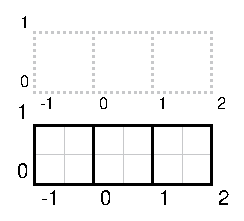
\includegraphics[width=0.5\textwidth]{eps_figure.eps}
   \end{figure}
\end{frame}

\begin{frame}[fragile]\frametitle{插入pdf图片}
   \begin{block}{Input}
    \begin{verbatim}
    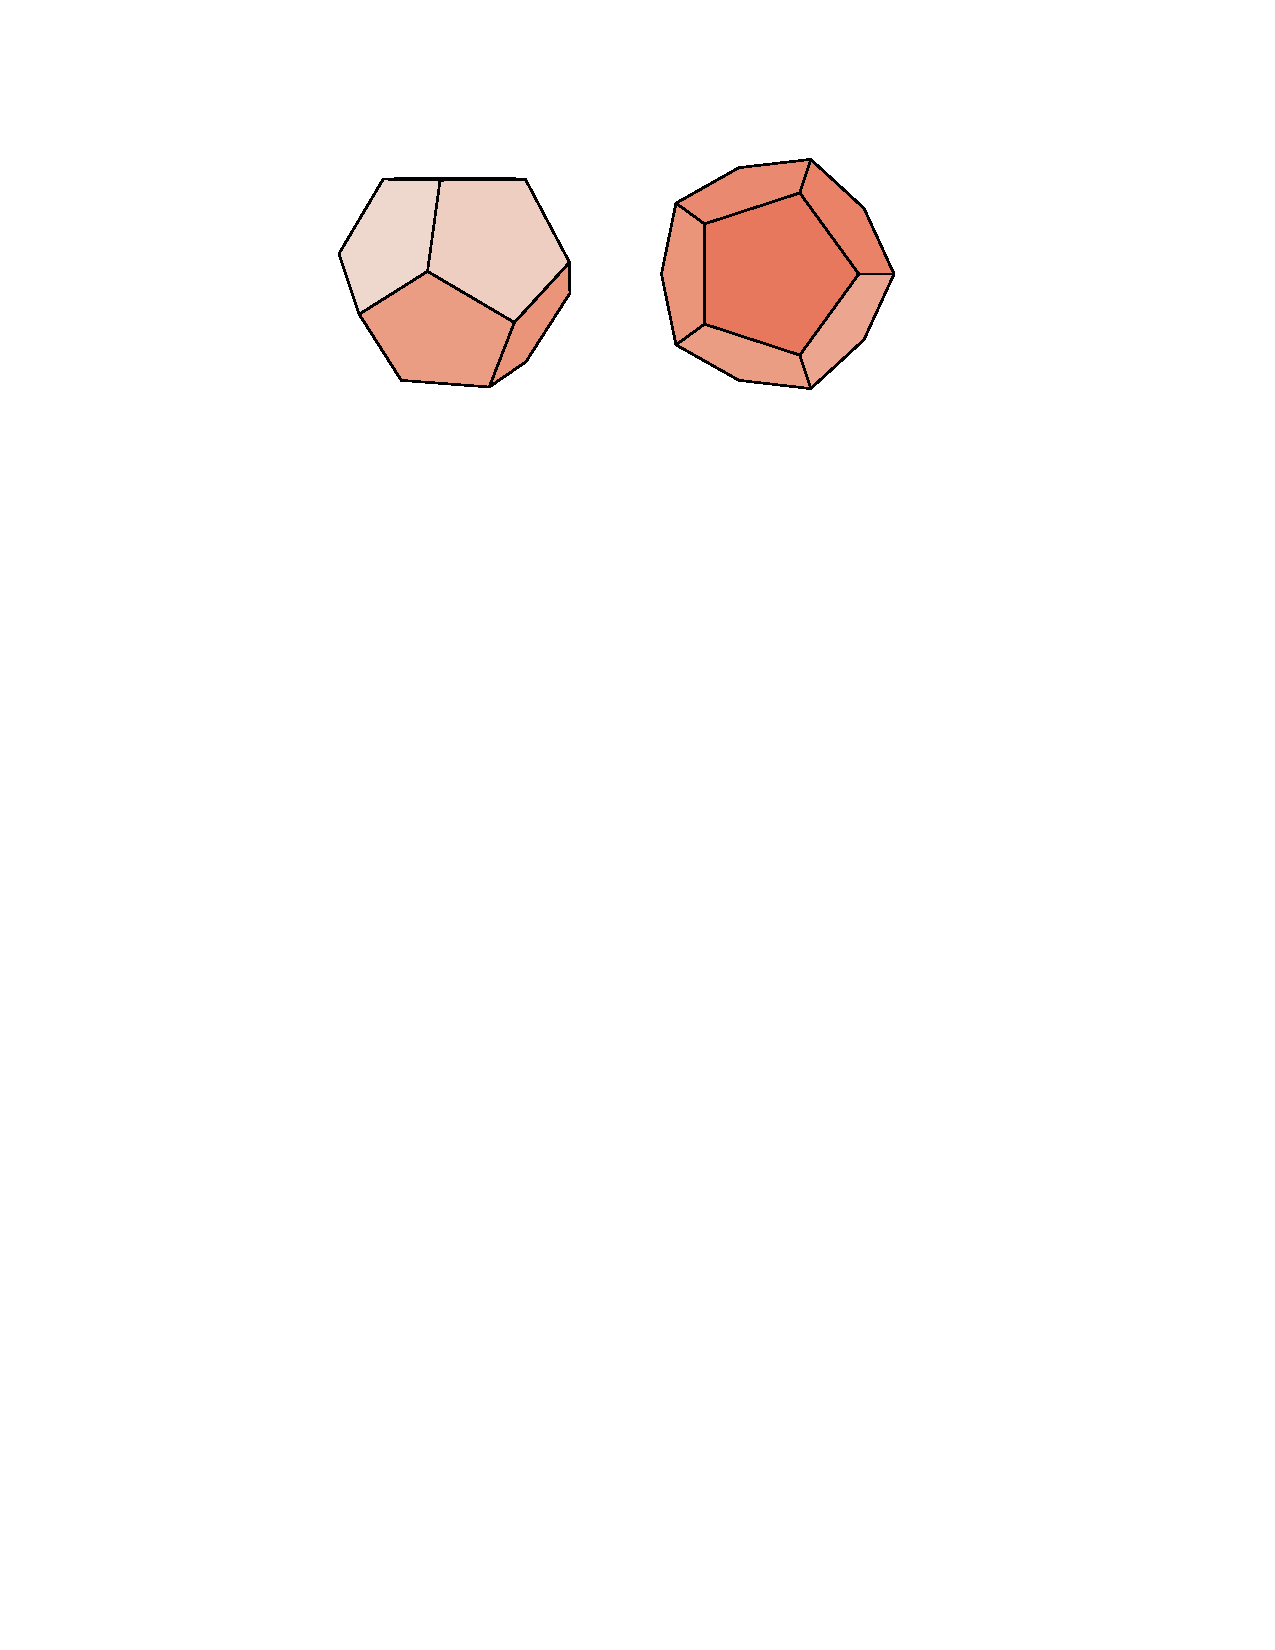
\includegraphics[width=0.5\textwidth]{pdf_figure.pdf}
    \end{verbatim}
   \end{block}
   \begin{figure}[h]
    \centering
    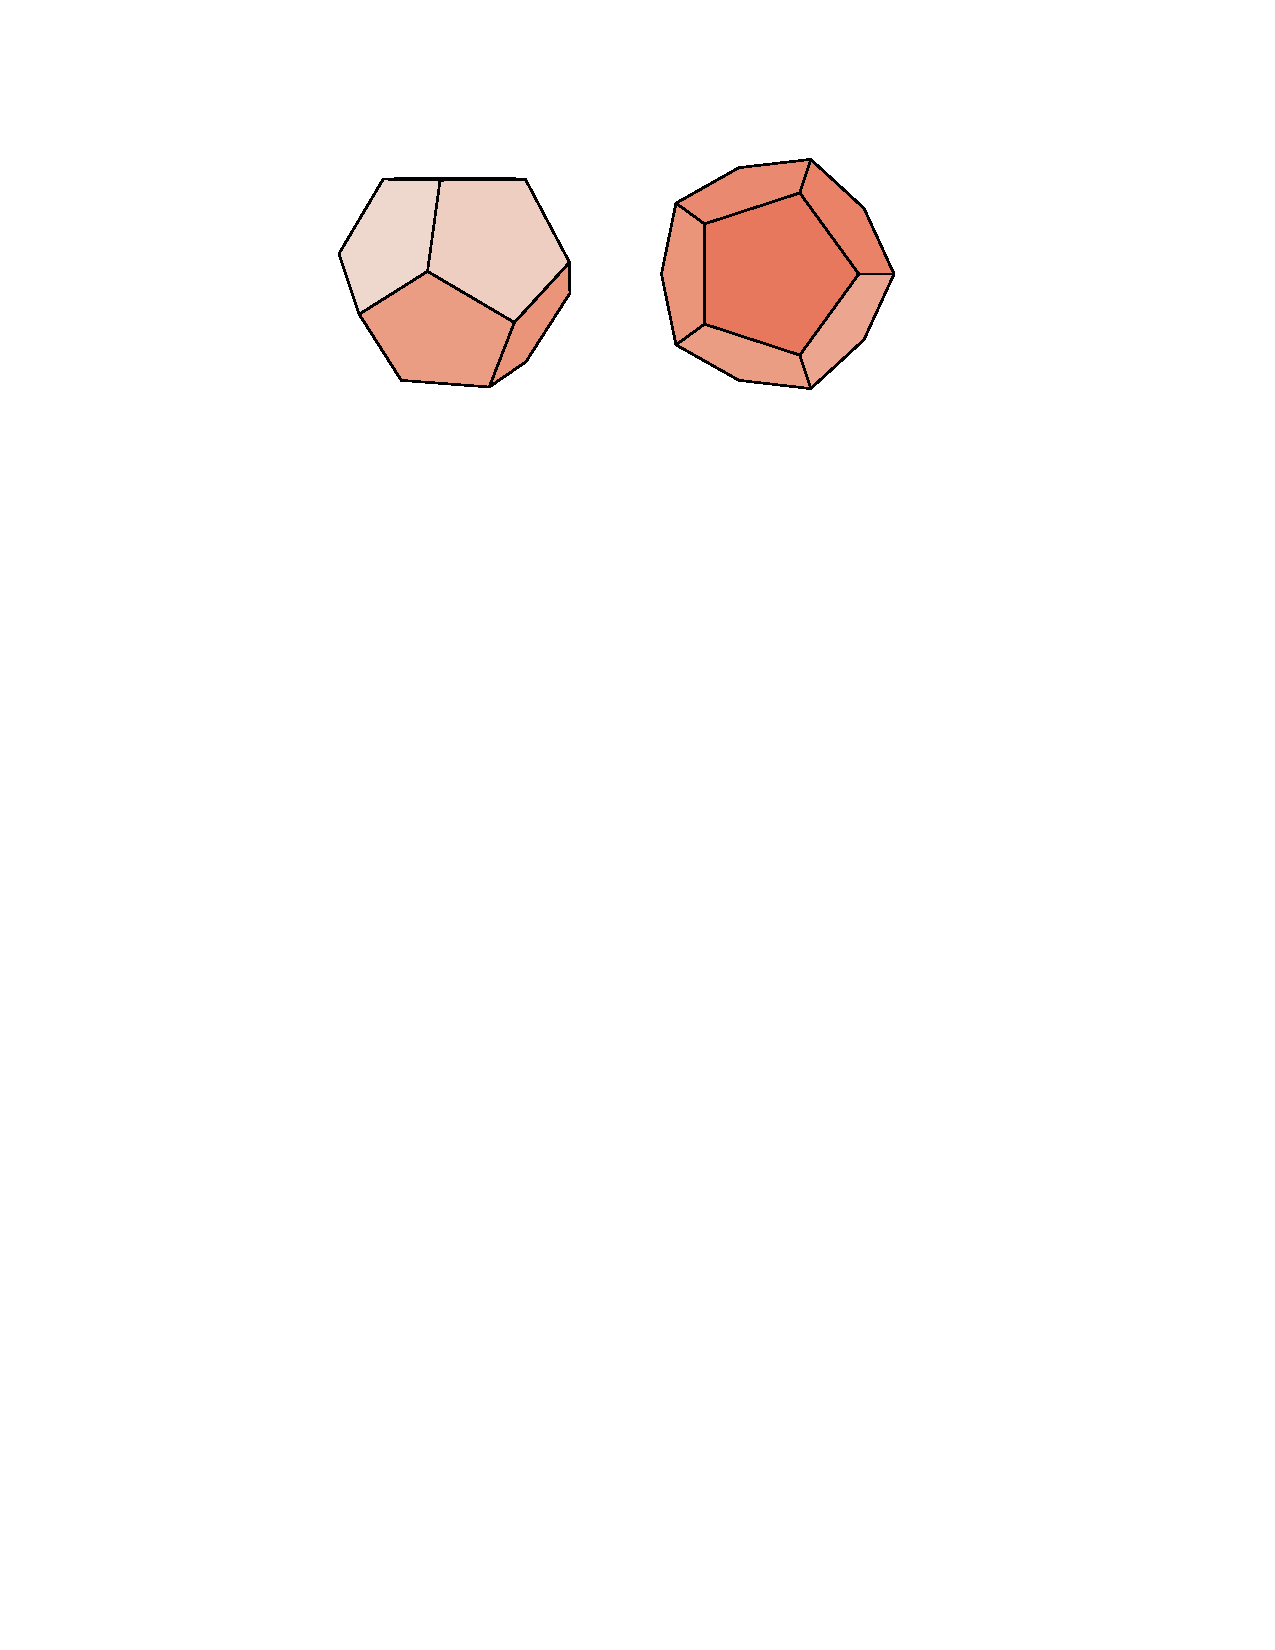
\includegraphics[width=0.5\textwidth]{pdf_figure.pdf}
   \end{figure}
\end{frame}

\begin{frame}\frametitle{插入MetaPost}
   \begin{figure}[h]
    \centering
    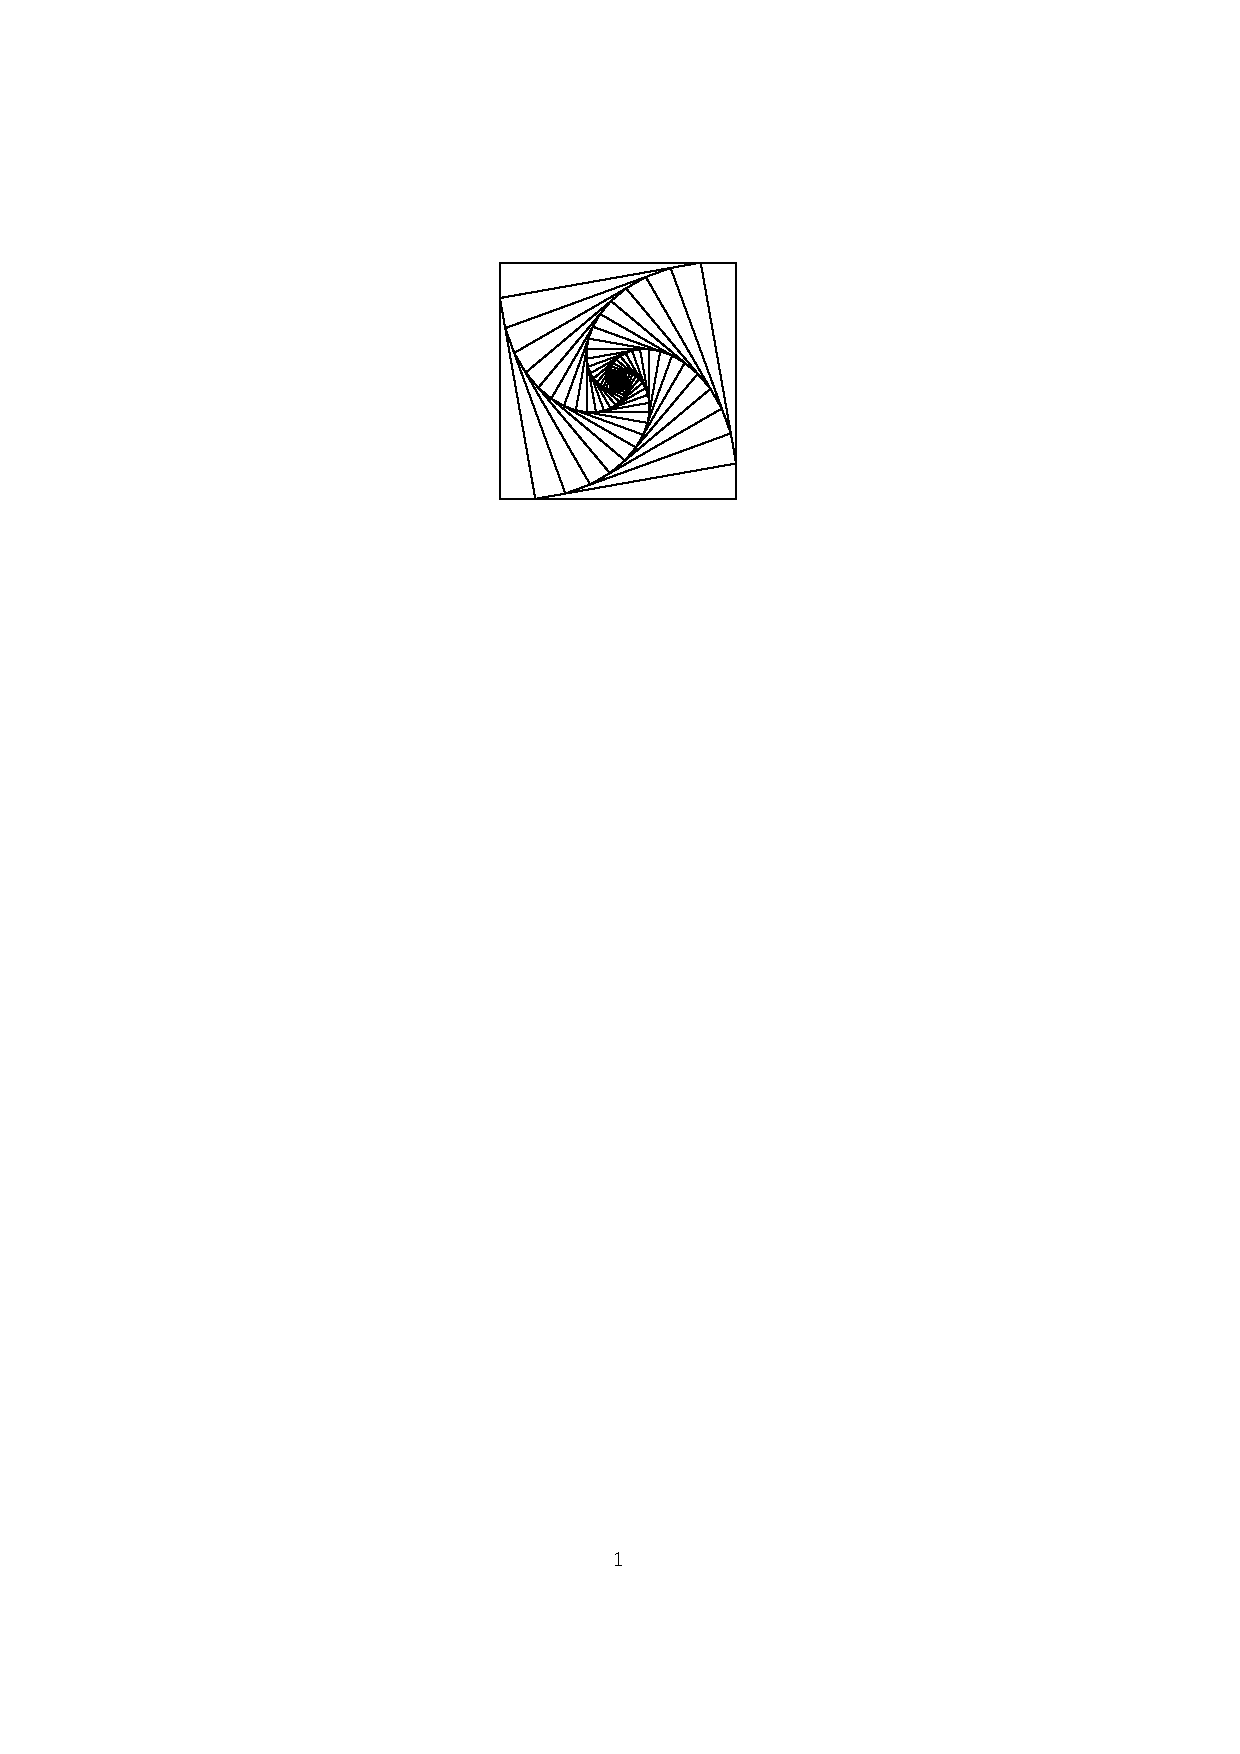
\includegraphics[width=1\textwidth]{metapost_figure}
   \end{figure}
\end{frame}

\begin{frame}\frametitle{插入TikZ}
   \begin{figure}\setcounter{subfigure}{0}
    \centering
    \subfigure[$G$~(无向图)]{\begin{tikzpicture}
    \tikzstyle{every node}=[inner sep=1pt,circle,draw,fill=black!25,scale=0.7]
    \path (0,0) node(3) {$v_3$}
          (-1,1.4) node(2) {$v_2$}
          (0.3,3) node(1) {$v_1$}
          (1.4,0.7) node(4) {$v_4$}
          (1.5,2) node(5) {$v_5$};
    \foreach \source/\target in {1/2, 2/3, 3/4, 4/2}
    \draw[orange,line width=1.4pt] (\source) --(\target);
    \end{tikzpicture}}\qquad
    \subfigure[$G'$~(有向图)]{\begin{tikzpicture}
    \tikzstyle{every node}=[inner sep=1pt,circle,draw,fill=black!25,scale=0.7]
    \path (0,0) node(3) {$v_3'$}
          (-1.2,1.7) node(2) {$v_2'$}
          (0.3,3) node(1) {$v_1'$}
          (1.3,1.2) node(4) {$v_4'$};
    \foreach \source/\target in {1/2, 2/3, 3/1, 4/2, 1/4}
    \draw[->,orange,line width=1.4pt] (\source) --(\target);
    \end{tikzpicture}}\qquad
    \subfigure[$G''$~(混合图)]{\begin{tikzpicture}
    \tikzstyle{every node}=[inner sep=1pt,circle,draw,fill=black!25,scale=0.7]
    \path (0,0) node(3) {$v_3''$}
          (0.3,2) node(2) {$v_2''$}
          (2.5,0.3) node(1) {$v_1''$}
          (2,2.3) node(4) {$v_4''$};
    \foreach \source/\target in {1/3, 3/4}
    \draw[->,orange,line width=1.4pt] (\source) --(\target);
    \draw[orange,line width=1.4pt] (2) --(4);
    \draw[orange,line width=1.4pt] (1) --(4);
    \end{tikzpicture}}
    \end{figure}
\end{frame}


\begin{frame}[fragile]\frametitle{引用}
  \begin{columns}
    \begin{column}{0.01\textwidth}
    \end{column}
    \begin{column}{0.55\textwidth}
    \begin{block}{Input}
    \begin{verbatim}
\begin{equation}
\lim_{x \to 0}\frac{\sin x}{x}=1
\label{myequation}
\end{equation}
(\ref{myequation})式是一个很重要的极限
    \end{verbatim}
    \end{block}
    \end{column}
    \begin{column}{0.025\textwidth}
    \end{column}
    \begin{column}{0.4\textwidth}
    \begin{block}{Output}
        \begin{equation}
        \lim_{x \to 0}\frac{\sin x}{x}=1
        \label{myequation}
        \end{equation}
        (\ref{myequation})式是一个很重要的极限
    \end{block}
    \end{column}
    \begin{column}{0.015\textwidth}
    \end{column}
  \end{columns}
\end{frame}


%************************************************
\section{中文支持}
\begin{frame}\frametitle{中文支持}
    \begin{itemize}
        \item<1-> CJK
            \begin{itemize}
              \item<2-> 一个德国人开发的中、日、韩文字处理包
              \item<3-> 是 \LaTeX{} 系统的一个宏包,比较通用
            \end{itemize}
        \item<4-> CCT
            \begin{itemize}
              \item<5-> 中科院张林波教授开发的中文系统
              \item<6-> 中文字体比较多,排版方式考虑中文使用习惯
              \item<7-> 缺点是需要进行预处理,引入其它LaTeX资源时会有一些问题
            \end{itemize}
        \item<8-> 天元
            \begin{itemize}
              \item<9-> 华东师大的肖刚、陈志杰等开发的中文 \TeX{}系统
            \end{itemize}
        \item<10-> \XeLaTeX{}
            \begin{itemize}
              \item<11-> 从底层支持中文
            \end{itemize}
    \end{itemize}
\end{frame}

\begin{frame}[fragile]\frametitle{CJK中文支持}
\begin{block}{CJK格式}
    \begin{verbatim}
\documentclass{article}
\usepackage{CJK}
\begin{document}
\begin{CJK*}{GBK}{kai}
这是中文楷体字。
\end{CJK*}
\end{document}
    \end{verbatim}
\end{block}
\end{frame}

\begin{frame}[fragile]\frametitle{CCT中文支持}
\begin{block}{老版本CCT格式}
    \begin{verbatim}
\documentclass{cctart}
\begin{document}
\kaishu 这是中文楷体字。
\end{document}
    \end{verbatim}
\end{block}

\begin{block}{新版本CCT格式}
    \begin{verbatim}
\documentclass[CJK]{cctart}
\begin{document}
\kaishu 这是中文楷体字。
\end{document}
    \end{verbatim}
\end{block}
\end{frame}

\begin{frame}[fragile]\frametitle{\XeLaTeX{} 中文支持}
\begin{block}{\XeLaTeX{} 格式1 (编码保存为UTF-8)}
    \begin{verbatim}
\documentclass{ctexart}
\begin{document}
中文宏包测试
\end{document}
    \end{verbatim}
\end{block}

\begin{block}{\XeLaTeX{}格式2}
    \begin{verbatim}
\documentclass{article}
\usepackage{ctex}
\begin{document}
中文宏包测试
\end{document}
    \end{verbatim}
\end{block}
\end{frame}


%************************************************
\section{Beamer}
\begin{frame}\frametitle{Beamer简介}
Beamer 是一个用于制作演示文稿的LaTeX 文档类,由Till
Tantau 编写。相对于其它同类工具,Beamer 有如下这些优点:
\begin{itemize}
    \item<2-> \textcolor{red}{标准统一}。标准的 \LaTeX{} 指令在 Beamer 文稿中可直接使用;
    \item<3-> \textcolor{red}{主题丰富}。提供了许多主题 (theme),可以很容易改善简档的外观;
    \item<4-> \textcolor{red}{注重内容}。致力于更好的表现演讲内容,而不是仅仅为了让页面好看;
    \item<5-> \textcolor{red}{方便定制}。页面布局、色彩、字体都可以实现全局调控;
\end{itemize}
\end{frame}

\begin{frame}[fragile]\frametitle{hello\_beamer.tex}
\begin{block}{}
    \begin{verbatim}
\documentclass{beamer}
\begin{document}
\begin{frame}
Hello Beamer!
\end{frame}%
\end{document}
    \end{verbatim}
\end{block}
从这个例子可以看出,Beamer 中每张幻灯片的内容都是放置在一个frame 环境里面的。
\end{frame}

\begin{frame}[fragile]\frametitle{hello\_beamer\_CN.tex}
\begin{block}{}
    \begin{verbatim}
\documentclass{beamer}
\usepacakge[UTF8]{ctex}
\begin{document}
\begin{frame}
你好Beamer!
\end{frame }
\end{document}
    \end{verbatim}
\end{block}
对于中文文档,建议用UTF8 编码,然后用xelatex 程序编译。
另外,可以在载入ctex 宏包时加上noindent 选项以取消段落
的缩进。
\end{frame}

\begin{frame}[fragile]\frametitle{Beamer基本语法}
\begin{block}{}
    \begin{verbatim}
\begin{frame}{幻灯片标题}{我是一个副标题}
Hello Beamer!
\end{frame }
    \end{verbatim}
\end{block}
或者
\begin{block}{}
    \begin{verbatim}
\begin{frame}
\frametitle{幻灯片标题}
\framesubtitle{我是一个副标题}
Hello Beamer!
\end{frame }
    \end{verbatim}
\end{block}
\end{frame}

\begin{frame}[fragile]\frametitle{Beamer文档结构}
在Beamer文档中,最常用的分节命令是\textbackslash section:
\begin{block}{}
    \begin{verbatim}
\section{Section Name}
    \end{verbatim}
\end{block}
类似于标题页面,我们可以在幻灯片中用\textbackslash tableofcontents 命令生成目录页。
\begin{block}{}
    \begin{verbatim}
\begin{frame}
\tableofcontents[hideallsubsections]
\end{frame }
    \end{verbatim}
\end{block}
其中hideallsubsections 选项表示不显示小节标题。
\end{frame}

\begin{frame}[fragile]\frametitle{简单的列表环境}
\begin{block}{}
    \begin{verbatim}
\begin{itemize}
\item<1-> 我是第一项
\item<2-> 我是第二项
\item<3-> 我是第三项
\end{itemize}
    \end{verbatim}
\end{block}
\begin{block}{}
\begin{itemize}
\item<1-> 我是第一项
\item<2-> 我是第二项
\item<3-> 我是第三项
\end{itemize}
\end{block}
\end{frame}

\begin{frame}[fragile]\frametitle{简单的区块环境}
\begin{block}{}
    \begin{verbatim}
\begin{block}{区块环境}
区块环境为了突出显示某些内容。
\end{block}
    \end{verbatim}
\end{block}
\begin{block}{区块环境}
区块环境为了突出显示某些内容。
\end{block}
\begin{alertblock}{警示区块环境}
警示区块环境为了警示突出某些内容。
\end{alertblock}
\begin{exampleblock}{例子区块环境}
例子区块环境为了突出例子内容。
\end{exampleblock}
\end{frame}

\begin{frame}\frametitle{beamer themes}
Beamer 的整体主题包含了结构、颜色、字体各方面的设置。
\begin{block}{}
\textbackslash usebeamertheme\{主题名\}
\end{block}
\begin{description}
    \item[无导航栏] 无导航栏default、boxes、Bergen、Pittsburgh 和 Rochester。
    \item[带顶栏] Antibes、Darmstadt、Frankfurt、JuanLesPins、Montpellier 和Singapore。
    \item[带底栏] Boadilla 和Madrid。
    \item[带顶栏底栏] AnnArbor、Berlin、CambridgeUS、Copenhagen、Dresden、Ilmenau、Luebeck、Malmoe、Szeged 和Warsaw。
    \item[带侧栏] Berkeley、Goettingen、Hannover、Marburg 和 PaloAlto。
\end{description}

\begin{center}
    \footnotesize{\url{http://deic.uab.es/~iblanes/beamer_gallery/}}
    \footnotesize{\url{http://www.hartwork.org/beamer-theme-matrix/}}
\end{center}
\end{frame}

\begin{frame}\frametitle{主题DIY}
Beamer 的各部分的内容都可以自己定制和修改,和主题的划分
类似,可以从如下这三个方面来定制自己的主题:

\begin{description}
    \item[定制模板] 用\textbackslash setbeamertemplate 命令
    \item[定制颜色] 用\textbackslash setbeamercolor 命令
    \item[定制字体] 用\textbackslash setbeamerfont 命令
\end{description}
\end{frame}


%************************************************
\section{参考文献}
\begin{frame}[fragile]\frametitle{参考文献}
主要介绍两种方法:
\begin{enumerate}
    \item<2-> 手工输入法
    \item<3-> \BibTeX{}
\end{enumerate}
\end{frame}

\begin{frame}[fragile]\frametitle{参考文献手工输入法}
\begin{block}{}
    \begin{verbatim}
As is stated in \cite{bibitem1} \dots
\begin{thebibliography}{9}
 \bibitem{bibitem1} 大傻瓜.如何做一个合格的大傻瓜[M].傻瓜帝国:傻瓜出版社.2013.
 \bibitem{bibitem2} 小傻瓜.如何成为一个大傻瓜[M].傻瓜帝国:傻瓜出版社.2013.
\end{thebibliography}
    \end{verbatim}
\end{block}
\begin{block}{}
As is stated in \cite{bibitem1} \dots
\begin{thebibliography}{9}
 \bibitem{bibitem1} 大傻瓜.如何做一个合格的大傻瓜[M].傻瓜帝国:傻瓜出版社.2013.
 \bibitem{bibitem2} 小傻瓜.如何成为一个大傻瓜[M].傻瓜帝国:傻瓜出版社.2013.
\end{thebibliography}
\end{block}
\end{frame}

\begin{frame}[fragile]\frametitle{传说中的高级玩法\BibTeX{}}
\BibTeX{} 是一个使用数据库的的方式来管理参考文献程序, 用于协调LaTeX的参考文献处理.
\begin{block}{}
    \begin{verbatim}
@article{Gettys90,
author = {Jim Gettys and Phil Karlton and Scott McGregor},
title = {The {X} Window System, Version 11},
journal = {Software Practice and Experience},
volume = {20},
year = {1990},
abstract = {A technical overview of the X11 functionality.}
}
    \end{verbatim}
\end{block}
\BibTeX{} 文件的后缀名为 .bib
\end{frame}

\begin{frame}[fragile]\frametitle{\LaTeX{}中用\BibTeX{}}
\begin{block}{}
    \begin{verbatim}
As is stated in \cite{fool} \dots
\bibliographystyle{plain}
\nocite{*}\bibliography{reference}
    \end{verbatim}
\end{block}
\begin{block}{}
    As is stated in \cite{fool} \dots
    \bibliographystyle{plain}
    \nocite{*}\bibliography{reference}
\end{block}
\end{frame}

\begin{frame}[fragile]\frametitle{\LaTeX{}中\BibTeX{}的编译流程}
\begin{block}{}
    \center
    \XeLaTeX{} $\color{red!70}\Longrightarrow{}$ \BibTeX{} $\color{red!70}\Longrightarrow$ \XeLaTeX{} $\color{red!70}\Longrightarrow$ \XeLaTeX{}
\end{block}
每步的解释:
\begin{enumerate}
    \item<2-> 用\XeLaTeX{} 编译你的 .tex 文件 , 这是生成一个 .aux 的文件, 这告诉\BibTeX{} 将使用那些引用
    \item<3-> 用\BibTeX{} 编译 .bib 文件 ,后台将 .bst文件和 .bib文件编译成 .bbl文件
    \item<4-> 再次用\XeLaTeX{} 编译你的 .tex 文件, 这个时候在文档中已经包含了参考文献, 但此时引用的编号可能不正确
    \item<5-> 最后用\XeLaTeX{} 编译你的 .tex 文件, 如果一切顺利的话, 这是所有东西都已正常了
\end{enumerate}
\end{frame}

\begin{frame}\frametitle{\BibTeX{}管理辅助软件}
如果要管理大量参考文献,就需要接下来讲的\BibTeX{}管理辅助软件了,这里我们主要介绍JabRef:
\begin{enumerate}
    \item<2-> 自动导入。支持CiteSeer、JSTOR、SPIRES、IEEEXplore、ArXiv.org、ACM Portal、Medline以及ScienceDirect 八大电子资源数据库的文献查找和索引自动导入功能。
    \item<3-> 转换方便。支持不同文献索引格式文件的导入和导出。可以广泛读取其他文献管理工具,如EndNote、Reference Manager、Refworks等保存的文献索引格式。
    \item<4-> 自动分类。支持任意分类和自动分类,可自动根据题目、作者、关键词或摘要自动分类。
    \item<5-> 兼容性强。支持在各种LaTex编辑器中和很多文本编辑器中插入文献记录,可以推送文献索引至写作文档。
\end{enumerate}
\end{frame} 

%************************************************
\section{几个有意思的工具}
\begin{frame}
  \frametitle{TeXFriend}
  \begin{enumerate}
    \item<2-> 南开大学孙文昌开发,WinEdt自带。
    \item<3-> TeXFrined提供几千个LaTeX字符的自动输入。
  \end{enumerate}
  \begin{center}
    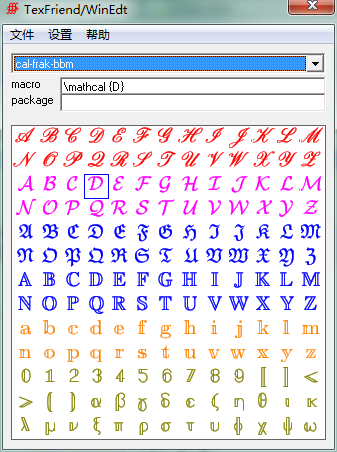
\includegraphics[width=0.4\textwidth]{texfriend.png}
  \end{center}
\end{frame}

\begin{frame}
  \frametitle{LYX}
  \begin{center}
    
\includegraphics[width=0.3\textwidth]{lyx.png}
  \end{center}
  \begin{enumerate}
    \item<2-> LyX是一个“所见即所指”(what you see is what you mean)的文件编辑软件。
    \item<3-> LyX利用\LaTeX{}来排版。
    \item<4-> 通过CJK-LyX提供中文支持。
    \item<5-> 可以生成\LaTeX{}文件和 PostScript 文件。
  \end{enumerate}
\begin{center}
    \footnotesize{\url{http://wiki.lyx.org/uploads/LyX/Screencasts/LyXIntroPalette.htm}}
\end{center}
\end{frame}

\begin{frame}
  \frametitle{Word2TeX}
  \begin{enumerate}
    \item<2-> 在Word中编辑文章
    \item<3-> 安装Word2TeX软件
    \item<4-> 将Word文档转化为TeX文件
    \item<5-> 对生成的TeX文件修改
    \item<6-> 再用LaTex编译为PDF文档
  \end{enumerate}
  \begin{center}
    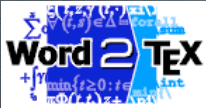
\includegraphics[width=0.3\textwidth]{word2tex.png} \qquad
    
\includegraphics[width=0.3\textwidth]{tex2word.png}
  \end{center}
\end{frame}

\begin{frame}
  \frametitle{巨人们的肩膀}
  \begin{enumerate}
    \item 中文\LaTeX{}安装与使用+"图论",\textcolor[rgb]{0.50,0.50,1.00}{黄正华}
    \item (仅供学习beamer参考之用),\textcolor[rgb]{0.50,0.50,1.00}{黄正华}
    \item 蔡老师\LaTeX{}简介入门,\textcolor[rgb]{0.50,0.50,1.00}{蔡炎龙}
    \item \XeLaTeX{}及WinEdt6.0入门指南,\textcolor[rgb]{0.50,0.50,1.00}{hy\_haoyun}
    \item 如何使用\LaTeX{}撰写科技论文,\textcolor[rgb]{0.50,0.50,1.00}{OSGeo讲座}
    \item WinEdt5.4 使用技巧,\textcolor[rgb]{0.50,0.50,1.00}{汤银才}
    \item 用\LaTeX{}排版编程技术书籍的一些个人经验,\textcolor[rgb]{0.50,0.50,1.00}{陈硕}
    \item \TeX{}/\LaTeX{}的使用和幻灯片的制作,\textcolor[rgb]{0.50,0.50,1.00}{谢歆}
    \item \LaTeX{}简介,\textcolor[rgb]{0.50,0.50,1.00}{唐国华师兄}
    \item Beamer 演示学习笔记,\textcolor[rgb]{0.50,0.50,1.00}{zoho}
    \item 一份不太简短的\LaTeX{}介绍,\textcolor[rgb]{0.50,0.50,1.00}{Tobias Oetiker}
  \end{enumerate}
\end{frame}

\begin{frame}
  \frametitle{谢谢大家}
  \begin{center}
    \Huge Q\&A?\\
    
\includegraphics[width=0.3\textwidth]{last}
  \end{center}
  \begin{center}
    才疏学浅,难免有错误之处,请大家谅解。\\同时欢迎发信交流,共同进步!\\
    \footnotesize{\LaTeX{}源文件:\url{https://github.com/lizekui/LatexIntro\#latexintro}}
  \end{center}
\end{frame}

\end{document} 